% =====================================================================
% MASTER VERSION -- long-form complete research record for advisor review.
% NOT optimised for a page limit. The 5-page submission version lives at
% paper/merged/haatim_hsgs_bounds_and_effective_rank.tex and is unaffected.
%
% DATA-HYGIENE NOTE, load-bearing for the whole document:
% three distinct experiment families appear here and are NEVER merged.
%   (B3)  results/track_b/b3/            via scripts/plot_paper.py
%         3 N x 2 pilot counts {10,30} x 6 SNR {-5..20}, 400 trials/point
%   (EXT) trackB_hankel_emgs/results/    via figure_array_size_comparison.py
%         P=30 only, 7 SNR {-10..20}, 600/400/200 trials at N=8/16/32
%   (TD)  results/track_d/partB9/        via scratch/trackD_partB9_*.py
%         adaptive order, 1 Cadzow sweep, SNR ~ U[-10,20], paired median
% Table II states all three. Every numeric claim carries a % SOURCE comment.
% =====================================================================
\documentclass[journal]{IEEEtran}
\IEEEoverridecommandlockouts

\usepackage{amsmath,amssymb,amsfonts}
\usepackage{algorithm}
\usepackage{algpseudocode}
\usepackage{graphicx}
\usepackage{booktabs}
\usepackage{url}
\usepackage[hidelinks]{hyperref}

\DeclareMathOperator{\rank}{rank}
\DeclareMathOperator{\range}{range}
\newcommand{\bG}{\mathbf{G}}
\newcommand{\bS}{\mathbf{S}}
\newcommand{\bB}{\mathbf{B}}
\newcommand{\bW}{\mathbf{W}}
\newcommand{\bZ}{\mathbf{Z}}
\newcommand{\bY}{\mathbf{Y}}
\newcommand{\bJ}{\mathbf{J}}
\newcommand{\bD}{\mathbf{D}}
\newcommand{\bU}{\mathbf{U}}
\newcommand{\bV}{\mathbf{V}}
\newcommand{\bH}{\mathbf{H}}
\newcommand{\bR}{\mathbf{R}}
\newcommand{\bg}{\mathbf{g}}
\newcommand{\bv}{\mathbf{v}}
\newcommand{\bw}{\mathbf{w}}
\newcommand{\CN}{\mathcal{CN}}
\newcommand{\Hank}{\mathcal{H}}
\newcommand{\reff}{r_{\mathrm{eff}}}
\newcommand{\rmax}{r_{\max}}
\newcommand{\dhs}{\Delta_{\mathrm{HS}}}
\newcommand{\jmathi}{\jmath}

\begin{document}

\title{Hankel-Structured Gerchberg--Saxton Channel Estimation for Rydberg
Atomic MIMO Receivers: Bounds, Aperture Scaling, Effective-Rank Normalisation,
and Prospective Cross-Generator Validation\\
\large\textnormal{(Master version --- complete research record for review)}}

\author{Abdullah~Haatim%
\thanks{A.~Haatim is with the Department of Electrical and Electronics
Engineering, Birla Institute of Technology and Science, Pilani~--- Pilani
Campus, India (e-mail: f20220519@pilani.bits-pilani.ac.in).}%
\thanks{\textbf{This is a long-form master version} assembled for advisor
review. It deliberately retains all defensible theory, methodology,
diagnostics, positive results, negative results and limitations, and is not
compressed to a conference page limit.}}

\maketitle

\begin{abstract}
Rydberg atomic receivers read out radio fields through an optical transition
whose response is proportional to field magnitude, so multi-user channel
estimation becomes a phase-retrieval problem with a known additive reference.
We first show that, under the unconstrained row-wise parameterisation of the
channel, the exact Rician Fisher information is block diagonal across receive
elements: each magnitude measurement contributes rank-one information, and the
per-element estimation problem is unchanged by adding elements. Increasing the
aperture therefore does not by itself increase normalised per-element
information for an unstructured estimator, and exploiting aperture requires
cross-element structure. On a uniform linear array the geometric multipath
model supplies exactly such structure: each path contributes one spatial
complex exponential, so the Hankel lifting of every channel column has rank at
most the path count. HS-GS enforces this by interleaving a Cadzow structured
low-rank projection with an exact expectation--maximisation Gerchberg--Saxton
iteration, selecting the model order from held-out pilots rather than an
oracle. Against a rank-one Rician Cram\'er--Rao bound and a
geometry-constrained bound on the $3\sum_k L_k$-parameter manifold, HS-GS
improves on EM-GS by $2.27$--$3.04$~dB at $N=32$, and its advantage grows with
aperture ($-0.19$, $+0.78$, $+2.85$~dB at $N=8,16,32$) while EM-GS moves by
$0.012$~dB. A controlled path-count sweep establishes the mechanism; replacing
raw path count by the effective Hankel rank relative to capacity generalises
it, giving a sign boundary near $\reff/\rmax\approx0.5$ that is stable to
within $0.07$ across $N\in\{16,32,64\}$ although the gain magnitude does not
collapse. Used prospectively and without refitting, that relation predicted the
gain on two previously unused channel generators. Negative results are retained
throughout: $N=8$ is a mixed result, the projection is approximate and
non-idempotent, the magnitude collapse is imperfect, a pre-registered
$K$-invariance falsifier is missed by $0.006$~dB, and the second prospective
prediction errs by $0.315$~dB. All results are simulation only, and neither
bound strictly governs the biased estimators compared against it.
\end{abstract}

\begin{IEEEkeywords}
Rydberg atomic receiver, channel estimation, phase retrieval, Hankel matrix,
structured low-rank approximation, constrained Cram\'er--Rao bound, effective
rank.
\end{IEEEkeywords}

% =====================================================================
\section{Introduction}
% =====================================================================

\IEEEPARstart{R}{ydberg} atomic receivers detect radio-frequency fields by
driving alkali atoms into highly excited states and reading the resulting
optical transmission. The measured quantity is proportional to the
\emph{magnitude} of the total incident field superposed on a known local
reference beam; the phase is not observed
\cite{cui2025,gong2025mag,zhang2024}. For a multi-user uplink this turns
channel estimation from a linear-Gaussian problem into a phase-retrieval
problem with a known additive offset.

Two families of solver exist for this. Alternating-projection methods of the
Gerchberg--Saxton type \cite{gerchberg1972} iterate between a measurement
constraint and a model constraint; the expectation--maximisation refinement
(EM-GS) replaces the hard magnitude substitution by the Rician posterior mean
and is the strongest classical baseline we are aware of for this observation
model. Separately, recent work unrolls such an iteration into a trained
network \cite{xiao2026}, and a rank projection has been placed inside projected
gradient descent for the same problem \cite{xu2025}.

\textbf{The gap.} All of these treat the channel matrix $\bG$ as an
unconstrained collection of parameters. That has a consequence which is easy to
miss and, once seen, organises the rest of this paper: under the unconstrained
row-wise parameterisation, row $n$ of $\bG\bS$ enters only measurement row $n$,
so the Fisher information is block diagonal across receive elements
(\S\ref{sec:crlb}). The per-element estimation problem is therefore unchanged
by adding elements, and \emph{a larger aperture does not by itself buy an
unstructured estimator anything under a normalised metric}. We measure exactly
this: EM-GS moves by $0.012$~dB across a fourfold change in $N$
(\S\ref{sec:aperture}).

Exploiting aperture consequently requires \emph{cross-element} structure. The
geometric multipath model on a uniform linear array (ULA) supplies one: each
propagation path contributes a single spatial complex exponential across the
array, so the Hankel lifting of each channel column is a sum of $L_k$ rank-one
terms and has rank at most $L_k$ (\S\ref{sec:hankel}). Enforcing that rank
inside the iteration is the method studied here, HS-GS. We emphasise at the
outset that Hankel structure is \emph{one} such cross-element structure and we
make no claim that it is the only one.

\textbf{Why effective rank becomes necessary.} A controlled experiment sweeping
the true path count $L$ establishes the mechanism cleanly
(\S\ref{sec:pathcount}). But $L$ is a parameter of one generator, not a
property of a channel, and it is a poor predictor across generators: a
$16$-path channel on a $32$-element array is algebraically full rank yet has an
effective Hankel rank of $8.73$, so its lifting is compressible with nothing
sparse about it. Replacing $L$ by the Roy--Vetterli effective rank
\cite{royvetterli2007} relative to the structural capacity gives a coordinate
that can be computed for any channel, and it is what makes the prospective
tests of \S\ref{sec:crossgen} possible.

\subsection{Contributions}

We separate these deliberately, and we do not claim novelty for the
ingredients individually --- Cadzow projection, EM-GS and constrained
Cram\'er--Rao bounds are all standard.

\begin{enumerate}
\item[\textbf{A.}] \textbf{Method.} HS-GS: a Cadzow structured low-rank
projection interleaved with an exact EM-GS iteration, with the model order
chosen from held-out pilots and no oracle path count anywhere. The magnitude
observation is never linearised. \S\ref{sec:method}.

\item[\textbf{B.}] \textbf{Analysis.} The exact Rician Fisher information for
this observation model, showing that each magnitude measurement contributes
\emph{rank-one} information rather than rank two, that the resulting matrix is
block diagonal across receive elements, and a geometry-constrained bound in
tangent-space form because the geometric parameterisation is rank deficient.
\S\ref{sec:crlb}.

\item[\textbf{C.}] \textbf{Mechanism.} Aperture scaling with an unstructured
baseline that is flat in $N$, plus a controlled path-count sweep in which the
gain decays monotonically to zero exactly as the prior becomes vacuous ---
which rules out generic denoising. \S\ref{sec:aperture},
\S\ref{sec:pathcount}.

\item[\textbf{D.}] \textbf{Generalisation.} Effective Hankel rank relative to
capacity as the structural coordinate, and an empirical sign boundary near
$\reff/\rmax\approx0.5$ that is stable across $N\in\{16,32,64\}$ ---
together with the explicit statement that the gain \emph{magnitude} does not
collapse onto the same axis. \S\ref{sec:effrank}, \S\ref{sec:boundary}.

\item[\textbf{E.}] \textbf{Validation.} Two prospective cross-generator
predictions, each registered in version control before the corresponding
measurement was run, using a stated interpolation rule that was not refitted
afterwards. \S\ref{sec:crossgen}.

\item[\textbf{F.}] \textbf{Robustness and limits.} A $K$-invariance test at
controlled pilot adequacy, the selector's abstention behaviour, and an explicit
catalogue of the regimes in which the method fails or the evidence is
incomplete. \S\ref{sec:kinv}, \S\ref{sec:limits}.
\end{enumerate}

% =====================================================================
\section{Related Work}
% =====================================================================

\textbf{Rydberg atomic receivers and magnitude-only estimation.} Cui \emph{et
al.} \cite{cui2025} formalise the atomic MIMO observation model in which the
receiver measures $|\bG\bS+\bB+\bW|$, and give the SNR and
reference-to-signal-ratio conventions we adopt. Overviews of the technology and
its sensing applications appear in \cite{gong2025mag,zhang2024}, and the
multi-user uplink is treated in \cite{gong2025icc}. \emph{These works establish
the measurement model; they do not impose channel structure inside the
estimator}, which is what this paper does.

\textbf{Phase retrieval and GS-type solvers.} The Gerchberg--Saxton iteration
\cite{gerchberg1972} is the classical alternating-projection method for
recovering phase from magnitude. Its EM refinement replaces the hard magnitude
substitution by the Rician conditional mean and is our baseline. \emph{Existing
GS/EM-GS treatments estimate an unconstrained signal}; we retain the exact
iteration and add a structural projection.

\textbf{Unrolled and rank-projected estimators.} Xiao \emph{et al.}
\cite{xiao2026} unroll a stabilised EM-GS into a trained network for this exact
receiver. Xu \emph{et al.} \cite{xu2025} place a rank projection inside
projected gradient descent and report that ``when the pilot length is small
($P=10$), the PGD performs better than the basic GD, as the projection
operation in PGD helps to exploit the rank constraint''. \emph{The distinction
that matters is which matrix is constrained}: their constraint applies to the
channel matrix of a two-dimensional ($8\times8$) array, limiting the number of
distinct spatial signatures across users; ours applies per user, to the Hankel
lifting of a single column, and encodes the harmonic structure of the ULA
manifold, so it is informative even at $K=1$. The two are complementary. They
are also not available at the same scale: their one-dimensional array has $I=8$
elements, for which $\rmax(8)=4$ by \eqref{eq:cap}, so the embedding admits at
most four ranks and the regime this paper characterises barely exists there.

\textbf{Structured low-rank approximation.} Cadzow's composite property mapping
\cite{cadzow1988} alternates projection onto fixed-rank matrices and onto
Hankel matrices; Markovsky \cite{markovsky2008} surveys the structured low-rank
approximation problem and its non-convexity. \emph{We use these as given} and
do not claim a new projection algorithm; our contribution is placing the
projection inside the exact phase-retrieval iteration and selecting its order
without an oracle.

\textbf{Constrained Cram\'er--Rao bounds.} Gorman and Hero \cite{gorman1990}
and Stoica and Ng \cite{stoica1998} give the constrained CRLB in the form we
require, which depends on a basis of the tangent space rather than on the
parameterisation itself --- necessary here because the geometric
parameterisation is rank deficient (\S\ref{sec:crlb}-B).

\textbf{Effective rank.} Roy and Vetterli \cite{royvetterli2007} define the
effective rank as the exponential of the spectral entropy of the normalised
singular values. \emph{We use it as a diagnostic coordinate}, not as a new
theoretical object.

\textbf{Channel model.} The clustered Saleh--Valenzuela model used in the
cross-generator tests follows the description in \cite{meijerink2014}, which is
the reference \cite{xiao2026} itself cites; the second configuration is taken
from the simulation section of \cite{precoding2408}, a precoding study by the
same group as \cite{cui2025}.

% =====================================================================
\section{System Model}\label{sec:model}
% =====================================================================

\subsection{Observation model}

An $N$-element ULA serves $K$ single-antenna users over $P$ pilot symbols. Let
$\bG\in\mathbb{C}^{N\times K}$ be the channel, $\bS\in\mathbb{C}^{K\times P}$
the pilot matrix, $\bB\in\mathbb{C}^{N\times P}$ the known reference beam and
$\bW\in\mathbb{C}^{N\times P}$ additive noise. The receiver observes
\begin{equation}\label{eq:obs}
\bZ=\bigl|\bG\bS+\bB+\bW\bigr|,\qquad \bW_{np}\sim\CN(0,\sigma^2),
\end{equation}
with $|\cdot|$ applied elementwise and $\bZ\in\mathbb{R}_{\ge0}^{N\times P}$.

Two properties of \eqref{eq:obs} are load-bearing. First, \textbf{the noise is
inside the modulus}: $\bZ$ is not a noisy observation of $|\bG\bS+\bB|$, and
each entry is Rice distributed rather than Gaussian. Second, \textbf{the
modulus is never linearised} anywhere in HS-GS or in either baseline; this is
checked per trial by the verification harness (\S\ref{sec:setup}).

\textbf{A terminological clarification.} Throughout, ``biased phase retrieval''
refers to the known reference-field offset $\bB$ in \eqref{eq:obs}. This is
entirely distinct from the \emph{statistical estimator bias} discussed in
\S\ref{sec:crlb}-C, which is why the Cram\'er--Rao bounds do not strictly
govern the estimators compared against them.

\subsection{Geometric ULA channel}

User $k$'s channel follows a sparse geometric multipath model with $L_k$ paths:
\begin{equation}\label{eq:chan}
g_k[n]=\sum_{\ell=1}^{L_k}\alpha_{\ell,k}\,e^{-\jmathi(n-1)\psi_{\ell,k}},
\qquad n=1,\dots,N,
\end{equation}
with, for half-wavelength element spacing,
\begin{equation}\label{eq:psi}
\psi_{\ell,k}=\pi\sin\theta_{\ell,k}.
\end{equation}
Equivalently $\bg_k=\sum_\ell\alpha_{\ell,k}\mathbf{a}(\theta_{\ell,k})$ with
$[\mathbf{a}(\theta)]_n=e^{-\jmathi\pi(n-1)\sin\theta}$.

The assumptions, stated so they can be attacked:
\begin{itemize}
\item \emph{Sparse geometric multipath.} $L_k$ is small relative to $N$; in the
principal experiments $L_k\sim\mathcal{U}\{3,\dots,7\}$~\cite{xu2025}.
\item \emph{Path gains.} $\alpha_{\ell,k}$ are i.i.d.\ circularly symmetric
complex Gaussian with equal expected power per path.
\item \emph{Angles of arrival.} $\theta_{\ell,k}$ i.i.d.\ uniform on
$(-90^\circ,90^\circ)$ in the principal generator. The cross-generator tests of
\S\ref{sec:crossgen} change this distribution and only this kind of thing.
\item \emph{Narrowband, flat.} No delay spread enters \eqref{eq:obs}.
\item \emph{Equal user power.} All users transmit at the same power; near--far
effects are untested (\S\ref{sec:limits}).
\item \emph{Pilots.} $\bS$ is drawn once per trial and shared bit-identically
by every estimator being compared (\S\ref{sec:setup}).
\end{itemize}

\subsection{SNR and RSR conventions}

SNR is defined at the array input in the usual sense. The
reference-to-signal ratio (RSR) is defined against a \emph{single} user, as in
\cite{cui2025}. Since $K$ users transmit simultaneously, a nominal single-user
RSR of $12$~dB corresponds to $12-10\log_{10}K=7.23$~dB against the $K$-user
total at $K=3$.
% SOURCE: trackB_hankel_emgs/config.py:18 (single-user denominator); arithmetic
% SOURCE: trackD_urformer/config.py:143-145 (empirical conversion 4.85 dB)
The empirically measured conversion is slightly larger than the nominal
$4.77$~dB --- $4.85$~dB over $300$ realisations --- which places the same case
at $7.15$~dB when measured rather than computed. The difference is
finite-sample; we quote nominal values and all RSR figures below are
single-user.

\subsection{Three experiment families, not one}

Results in this paper come from three distinct experiment families with
different configurations. \textbf{They are never pooled}, and every figure and
table below names the family it belongs to. Table~\ref{tab:params} gives the
model parameters and Table~\ref{tab:config} the per-family configurations.

\begin{table}[!t]
\caption{System and model parameters.}
\label{tab:params}
\centering
\begin{tabular}{ll}
\toprule
Symbol & Meaning / value \\
\midrule
$N$ & receive elements; $8,16,32$ (B3, EXT), $16,32,64$ (TD) \\
$K$ & users; $3$ unless swept ($2,3,4$ in \S\ref{sec:kinv}) \\
$P$ & pilot symbols; see Table~\ref{tab:config} \\
$\bG$ & $N\times K$ channel, columns as in \eqref{eq:chan} \\
$\bS$ & $K\times P$ pilots, shared across compared estimators \\
$\bB$ & $N\times P$ known reference beam \\
$\bW$ & $N\times P$ noise, $\CN(0,\sigma^2)$, inside the modulus \\
$L_k$ & paths per user, $\mathcal{U}\{3,\dots,7\}$~\cite{xu2025} \\
$\theta_{\ell,k}$ & AoA, $\mathcal{U}(-90^\circ,90^\circ)$ \\
$\rmax(N)$ & Hankel capacity $=\lceil N/2\rceil$, \eqref{eq:cap} \\
\bottomrule
\end{tabular}
\end{table}

\begin{table*}[!t]
\caption{The three experiment families. These are separate experiments with
different configurations and are never pooled.}
\label{tab:config}
\centering
\scriptsize
\setlength{\tabcolsep}{2pt}
\begin{tabular}{lllll}
\toprule
Family & Store / driver & Configuration & Statistic & Used in \\
\midrule
% SOURCE: results/track_b/b3/*.npz via scripts/plot_paper.py
\textbf{B3} (principal) & \texttt{results/track\_b/b3/} &
$N\in\{8,16,32\}$, $P\in\{10,30\}$, SNR $\{-5,0,5,10,15,20\}$, &
ratio-of-sums; per-point & Figs.~\ref{fig:snr},~\ref{fig:scaling}; \\
 & \texttt{scripts/plot\_paper.py} &
RSR $12$~dB, $T=50$, $n_{\mathrm{cz}}=4$; $400$ trials/point &
mean across points & \S\ref{sec:complexity},~\ref{sec:bounds},~\ref{sec:aperture} \\[1pt]
% SOURCE: trackB_hankel_emgs/results/ via figure_array_size_comparison.py
\textbf{EXT} (diagnostic) & \texttt{trackB\_hankel\_emgs/} &
$P=30$ only, SNR $\{-10,\dots,20\}$ (7 points), &
ratio-of-sums; mean of & Figs.~\ref{fig:panels},~\ref{fig:pathcount},~\ref{fig:spectrum},~\ref{fig:rawL}; \\
 & \shortstack[l]{\texttt{figure\_array\_size\_}\\\texttt{comparison.py}} &
RSR $12$~dB, $T=50$, $n_{\mathrm{cz}}=4$; $600/400/200$ trials &
per-SNR dB values & \S\ref{sec:aperture}-C,~\ref{sec:pathcount},~\ref{sec:spectrum} \\[2pt]
% SOURCE: results/track_d/partB9/ via scratch/trackD_partB9_sweeps.py
\textbf{TD} (effective rank) & \texttt{results/track\_d/partB9/} &
$N\in\{16,32,64\}$, $P=20$, SNR $\sim\mathcal{U}[-10,20]$, &
paired per-trial median, & Figs.~\ref{fig:boundary},~\ref{fig:crossgen},~\ref{fig:kinv}; \\
 & \texttt{scratch/trackD\_partB9\_sweeps.py} &
RSR $10$~dB, $T=100$, $n_{\mathrm{cz}}=1$, adaptive order &
bootstrap CI & \S\ref{sec:boundary}--\ref{sec:kinv} \\
\bottomrule
\end{tabular}
\end{table*}

% =====================================================================
\section{Why Hankel Structure Exists}\label{sec:hankel}
% =====================================================================

Drop the user index and write one channel column as
$g_n=\sum_{\ell=1}^{L}\alpha_\ell z_\ell^{\,n}$ with
$z_\ell=e^{-\jmathi\psi_\ell}$. Define the Hankel lifting with pencil parameter
$p$,
\begin{equation}\label{eq:lift}
\Hank(\bg)=
\begin{bmatrix}
g_0 & g_1 & \cdots & g_{p}\\
g_1 & g_2 & \cdots & g_{p+1}\\
\vdots & & \ddots & \vdots\\
g_{N-p-1} & \cdots & & g_{N-1}
\end{bmatrix}
\in\mathbb{C}^{(N-p)\times(p+1)}.
\end{equation}
Its $(q,r)$ entry is $g_{q+r}$, which separates in $q$ and $r$:
\begin{equation}\label{eq:sep}
\bigl[\Hank(\bg)\bigr]_{q,r}=\sum_{\ell=1}^{L}\alpha_\ell z_\ell^{\,q+r}
=\sum_{\ell=1}^{L}\alpha_\ell\,z_\ell^{\,q}\,z_\ell^{\,r}.
\end{equation}
With $\bv_\ell=[1,z_\ell,\dots,z_\ell^{N-p-1}]^{T}$ and
$\bw_\ell=[1,z_\ell,\dots,z_\ell^{p}]^{T}$ this is
\begin{equation}\label{eq:rank1}
\Hank(\bg)=\sum_{\ell=1}^{L}\alpha_\ell\,\bv_\ell\bw_\ell^{T},
\end{equation}
a sum of $L$ rank-one terms, hence
% SOURCE: derivation, this section
\begin{equation}\label{eq:rank}
\rank\bigl(\Hank(\bg)\bigr)\le L.
\end{equation}

Each propagation path creates one spatial complex exponential across the ULA
and therefore contributes exactly one rank-one component to the lifting. Three
consequences deserve emphasis.

\emph{When equality holds.} If the $z_\ell$ are distinct and $L$ does not
exceed either matrix dimension, \eqref{eq:rank} holds with equality; conversely
a sequence whose Hankel matrix has rank $L$ is a sum of $L$ exponentials
\cite{cadzow1988}.

\emph{Closely spaced paths.} If two $z_\ell$ are nearly equal the corresponding
rank-one terms are nearly collinear, so the matrix is only \emph{numerically}
rank deficient: the spectrum decays rather than terminating in an exact cliff.
This is precisely the regime the clustered generator of \S\ref{sec:crossgen}
creates, and it is why raw path count eventually fails as a predictor
(\S\ref{sec:effrank}).

\emph{Grid-free, and no angle estimation.} The constraint is on the rank of
\eqref{eq:lift}, not on coefficients over a discretised angular dictionary. No
$\theta_{\ell,k}$ is ever estimated, and no basis mismatch is possible.

\subsection{Structural capacity}

Since $\Hank(\bg)$ is $(N-p)\times(p+1)$, its rank cannot exceed
$\min(N-p,p+1)$, maximised over $p$ at
% SOURCE: derivation; verified by brute force against
% rydberg_sim/track_b_proposed.py:105 for N in {7,8,15,16,31,32,63,64}
\begin{equation}\label{eq:cap}
\rmax(N)=\max_{1\le p\le N-1}\min(N-p,\,p+1)=\bigl\lceil N/2\bigr\rceil,
\end{equation}
attained at $p=\lfloor N/2\rfloor$. Thus
\begin{center}
$\rmax(8)=4$, \quad $\rmax(16)=8$, \quad $\rmax(32)=16$, \quad $\rmax(64)=32$.
\end{center}
The ceiling, not the floor: at $N=7$ the maximum is $4$, and the two
expressions coincide only for even $N$.

If $\hat L\ge\rmax$ then $\rank\le\hat L$ holds for \emph{every} length-$N$
vector, so the constraint carries no information whatever and the projection
is the identity map. The capacity therefore states precisely \emph{when} the
prior can be informative, and it is the natural denominator for any rank-like
quantity --- which is the role it plays in \S\ref{sec:effrank}.

\subsection{Degrees-of-freedom motivation, and what it does not prove}

Treated as unstructured, $\bG$ has $2NK$ real degrees of freedom. Under
\eqref{eq:chan} it is described by approximately $3\sum_k L_k$ real parameters
(two per complex gain, one per angle). With $L_k\equiv\bar L$ the compression
ratio is
% SOURCE: derivation; verified numerically for (K,Lbar) in {2,3,4,6}x{3,5,7}
\begin{equation}\label{eq:compress}
\frac{3\sum_k L_k}{2NK}=\frac{3K\bar L}{2NK}=\frac{3\bar L}{2N},
\end{equation}
in which $K$ cancels.

\textbf{What this motivates and what it does not.} It motivates the hypothesis
that the structural gain should be invariant in $K$ once pilot adequacy is held
fixed, because the projection acts per user column and the compression
available per column does not depend on how many columns there are. It does
\emph{not} prove that hypothesis: a parameter count says nothing about
estimation error, the bound geometry, or the behaviour of a particular
iterative algorithm. \S\ref{sec:kinv} tests it directly, and the test partially
fails.

% =====================================================================
\section{The HS-GS Estimator}\label{sec:method}
% =====================================================================

\subsection{Exact EM-GS measurement update}

Let $\boldsymbol{\Lambda}=\bG\bS+\bB$ be the current noiseless-field estimate.
Conditional on it, each observation $z$ is Rice distributed with non-centrality
$a=|\lambda|$, and the conditional mean of the complex field is obtained by
scaling the observed magnitude by the Bessel ratio $R(x)=I_1(x)/I_0(x)$
evaluated at $\kappa=2za/\sigma^2$. Algorithm~\ref{alg:emgs} states one
iteration. The row-wise least squares in line~4 is exactly the structure that
makes the Fisher information block diagonal (\S\ref{sec:crlb}-A).

\begin{algorithm}[!t]
\caption{EM-GS measurement update $\mathcal{T}_{\mathrm{EM}}$ (one iteration)}
\label{alg:emgs}
\begin{algorithmic}[1]
\Require $\bZ,\bS,\bB,\sigma^2$; iterate $\bG$ ($\varnothing\Rightarrow$ spectral init)
\State $\boldsymbol{\Lambda}\leftarrow\bG\bS+\bB$;\quad
       $\boldsymbol{\kappa}\leftarrow(2/\sigma^2)\,\bZ\odot|\boldsymbol{\Lambda}|$
\State $\bR\leftarrow R(\boldsymbol{\kappa})$, $R(x)=I_1(x)/I_0(x)$
       \Comment{elementwise}
\State $\hat\bY\leftarrow\bR\odot\bZ\odot e^{\jmathi\angle\boldsymbol{\Lambda}}$
       \Comment{Rician posterior mean}
\State $\bG_{n,:}\leftarrow(\hat\bY_{n,:}-\bB_{n,:})\bS^{H}(\bS\bS^{H})^{-1}$,
       $n=1..N$ \Comment{rows independent}
\State \Return $\bG$
\end{algorithmic}
\end{algorithm}

\subsection{Cadzow projection}

Let $\mathcal{S}_{\hat L}$ be the set of length-$N$ sequences whose Hankel
lifting has rank at most $\hat L$. Membership is the intersection of two sets
that each admit an exact projector: fixed-rank matrices (truncated SVD,
Frobenius-optimal by Eckart--Young) and Hankel matrices (anti-diagonal
averaging). Cadzow's algorithm \cite{cadzow1988} alternates them
(Algorithm~\ref{alg:cadzow}).

\textbf{The projection is approximate, and we do not hide this.} The
intersection is a non-convex variety. The composite map
\begin{equation}\label{eq:notproj}
\mathcal{P}_{\hat L}=\Hank^{\dagger}\circ\Pi_{\hat L}\circ\Hank
\end{equation}
is \emph{not} in general an idempotent projection onto that intersection: one
application lands near, but not on, the set, and iterating changes the result.
This is why $n_{\mathrm{cz}}=4$ sweeps are used rather than one --- more sweeps
move closer to the intersection --- and why no convergence guarantee is claimed
for the outer iteration. \S\ref{sec:spectrum} quantifies the residual
directly: after four sweeps the singular-value cliff is restored only to
$\sim\!10^{-3}$, against $\sim\!10^{-16}$ for the true channel.

When $\hat L\ge\rmax$ the routine returns its input unchanged, so HS-GS then
reproduces EM-GS bit for bit (Algorithm~\ref{alg:cadzow}, line~2).

\begin{algorithm}[!t]
\caption{Cadzow projection $\mathcal{P}_{\hat L}$ of one channel column}
\label{alg:cadzow}
\begin{algorithmic}[1]
\Require $\bg\in\mathbb{C}^{N}$, rank $\hat L$, sweeps $n_{\mathrm{cz}}$
\State $p\leftarrow\arg\max_{p}\min(N-p,p+1)$;\quad
       $\rmax\leftarrow\lceil N/2\rceil$
\If{$\hat L\ge\rmax$} \Return $\bg$
       \Comment{constraint vacuous: exact no-op} \EndIf
\For{$t=1..n_{\mathrm{cz}}$}
  \State $\bH\leftarrow\Hank(\bg)$, $\bH_{q,r}=g_{q+r}$
         \Comment{$(N{-}p)\times(p{+}1)$}
  \State $\bU\boldsymbol{\Sigma}\bV^{H}\leftarrow\mathrm{svd}(\bH)$;\ \
         $\bH\leftarrow\bU_{:,1:\hat L}\boldsymbol{\Sigma}_{1:\hat L}
         \bV_{:,1:\hat L}^{H}$ \Comment{rank}
  \State $g_m\leftarrow|\mathcal{A}_m|^{-1}\!\!\sum_{(q,r)\in\mathcal{A}_m}\!\!\bH_{q,r}$,
         $\mathcal{A}_m\!=\!\{q{+}r{=}m\}$ \Comment{Hankel}
\EndFor
\State \Return $\bg$
\end{algorithmic}
\end{algorithm}

\subsection{Interleaved iteration}

The projection acts \emph{inside} the exact iteration, not as post-processing:
\begin{equation}\label{eq:map}
\bG^{(t)}=\mathcal{P}_{\hat L}\circ\mathcal{T}_{\mathrm{EM}}
\bigl(\bG^{(t-1)}\bigr),\qquad t=1,\dots,T,
\end{equation}
with $\mathcal{P}_{\hat L}$ applied column-wise after every one of the $T$
updates.

\textbf{Why inside rather than after.} The EM-GS update quality depends on the
current iterate through $\kappa=2z|\lambda|/\sigma^2$: the Bessel ratio is
evaluated at the current field estimate, so a structurally cleaner iterate
produces a better phase estimate, hence a better next iterate. Post-processing
a converged unstructured estimate cannot recover this compounding, because the
phase estimates that produced it were never improved.

\subsection{Held-out order selection}

HS-GS needs a target rank $\hat L$, and the true $L_k$ is unknown to any
practical receiver.

\textbf{The in-sample residual cannot supply it.} Constraining $\bG$ can only
worsen the fit to the pilots used for fitting, so an in-sample criterion always
prefers the largest candidate and the selector would degenerate to
$\hat L=\rmax$, i.e.\ to EM-GS. Holding out a validation fraction $\nu=0.3$ of
the pilot columns penalises over-modelling correctly, and every quantity
involved is observable:
\begin{equation}\label{eq:order}
\hat L=\arg\min_{1\le L\le \rmax}
\bigl\|\,\bZ_{\mathcal{V}}-\bigl|\bG_L\bS_{\mathcal{V}}
+\bB_{\mathcal{V}}\bigr|\,\bigr\|_F^{2},
\end{equation}
with $\bG_L$ the estimate at order $L$ from the fitting columns only, run for
$T_{\mathrm{sel}}=20$ iterations. \textbf{No oracle rank is used anywhere in
this paper.}

\textbf{The selector returns one scalar shared by all $K$ users}, which is a
limitation we state rather than defend (\S\ref{sec:limits}). Order matters both
ways: $\hat L<L$ truncates genuine components, a bias that does \emph{not}
vanish as noise decreases, while $\hat L>L$ admits noise and weakens the prior.
Ours systematically under-selects: true orders $(7,4,6)$ typically give
$\hat L=5$, and the mean $\hat L$ reaches only $11.63$ at $L=16$
% SOURCE: trackB_hankel_emgs/results/experiment_C_path_count.csv, mean_L_hat
(\S\ref{sec:pathcount}).

\textbf{Abstention.} When the selector returns $\hat L\ge\rmax$ the projection
is the identity and HS-GS reduces exactly to EM-GS. This is not a failure mode
but a designed one: the rule declines to impose structure it cannot support
from the held-out residual, without being told which channel it faces.
\S\ref{sec:crossgen} measures how often it does so on two different generators.

\begin{algorithm}[!t]
\caption{HS-GS, and the held-out rank selection it uses}
\label{alg:hsgs}
\begin{algorithmic}[1]
\Function{HS-GS}{$\bZ,\bS,\bB,\sigma^2$; $\hat L$, $T$}
  \State $\mathrm{active}\leftarrow(\hat L<\rmax)$;\quad $\bG\leftarrow\varnothing$
  \For{$t=1..T$}
    \State $\bG\leftarrow\mathcal{T}_{\mathrm{EM}}(\bG)$
           \Comment{Alg.~\ref{alg:emgs}: \emph{identical} to the baseline}
    \If{$\mathrm{active}$ \textbf{and} $t\bmod\Pi=0$}
      \State $\bG_{:,k}\leftarrow\mathcal{P}_{\hat L}(\bG_{:,k})$, $k=1..K$
             \Comment{Alg.~\ref{alg:cadzow}}
    \EndIf
  \EndFor
  \State \Return $\bG$
\EndFunction
\Statex
\Function{SelectRank}{$\bZ,\bS,\bB,\sigma^2$; $\nu$, $T_{\mathrm{sel}}$}
  \State $\mathcal{V}\leftarrow$ last $\lceil\nu P\rceil$ pilot columns;\quad
         $\mathcal{F}\leftarrow$ the rest
  \For{$L=1..\rmax$}
    \State $\bG_L\leftarrow\textsc{HS-GS}(\bZ_{:,\mathcal{F}},\bS_{:,\mathcal{F}},
           \bB_{:,\mathcal{F}},\sigma^2;L,T_{\mathrm{sel}})$
    \State $J(L)\leftarrow\|\bZ_{:,\mathcal{V}}-|\bG_L\bS_{:,\mathcal{V}}
           +\bB_{:,\mathcal{V}}|\|_F^{2}$
           \Comment{columns never fitted}
  \EndFor
  \State \Return $\hat L=\arg\min_L J(L)$
\EndFunction
\end{algorithmic}
\end{algorithm}

\textbf{Relation to the baseline.} Deleting lines 5--7 of
Algorithm~\ref{alg:hsgs} yields baseline EM-GS exactly: both chain the same
$\mathcal{T}_{\mathrm{EM}}$ for the same $T$ iterations from the same
initialisation, with no early stopping in either. Setting $\hat L\ge\rmax$
makes $\mathcal{P}_{\hat L}$ the identity, so the two then agree \emph{bit for
bit}; this is checked numerically (\S\ref{sec:setup}).

\subsection{Complexity}\label{sec:complexity}

One EM-GS update costs $O(NPK)$. The projection adds $Kn_{\mathrm{cz}}$ SVDs
per iteration, $O(Kn_{\mathrm{cz}}N^{3})$, and order selection multiplies this
by the $\rmax$ candidates.

Measured against a \emph{chained} EM-GS baseline --- the correct reference,
since HS-GS issues $T$ single-iteration calls --- HS-GS at fixed order costs
% SOURCE: results/track_b/timing.json, median_ms["hs_gs_fixed_L"] /
% median_ms["em_gs_chained"] = 1.492 / 1.322 / 1.216 at N = 8 / 16 / 32;
% order_search_share = 0.5773 / 0.7412 / 0.8550. This is a track_b timing
% run at the B3 configuration, NOT the EXT tree.
$1.49$, $1.32$, $1.22\times$ at $N=8,16,32$, so the ratio \emph{falls} with
$N$: the $O(N^3)$ SVD grows more slowly than the accumulated cost of the
baseline iteration at these sizes. Order selection dominates total runtime,
$57.7$--$85.5\%$, which makes the candidate set the obvious practical target
--- for instance a coarse-to-fine search, or reusing $\hat L$ across
coherence blocks. We describe this rather than pursue it.

% =====================================================================
\section{Exact Likelihood and Performance Bounds}\label{sec:crlb}
% =====================================================================

\subsection{Rank-one Fisher information}

Conditional on $\bG,\bS,\bB$ the noiseless field at $(n,p)$ is a known constant
$\lambda=(\bG\bS+\bB)_{n,p}$, so $z=|\lambda+w|$ is Rice distributed:
\begin{equation}\label{eq:rice}
p(z\mid\lambda)=\frac{2z}{\sigma^2}
\exp\!\Bigl(-\frac{z^2+|\lambda|^2}{\sigma^2}\Bigr)
I_0\!\Bigl(\frac{2z|\lambda|}{\sigma^2}\Bigr).
\end{equation}
Crucially \eqref{eq:rice} depends on $\lambda$ \emph{only through}
$a=|\lambda|$. Differentiating, with $\frac{d}{dx}\log I_0(x)=R(x)$,
\begin{equation}\label{eq:score}
\frac{\partial\log p}{\partial a}=\frac{2}{\sigma^2}\bigl[zR(\kappa)-a\bigr],
\qquad \kappa=\frac{2za}{\sigma^2}.
\end{equation}
Using the zero-mean-score identity $\mathbb{E}[zR(\kappa)]=a$ and writing
$\beta(a,\sigma^2)=\sigma^{-4}\bigl(\mathbb{E}[z^{2}R^{2}(\kappa)]-a^{2}\bigr)$,
one measurement carries scalar information
$I_a=\mathbb{E}[(\partial_a\log p)^2]=4\beta$. In real coordinates
$\boldsymbol{\eta}=[\Re\mathrm{vec}\,\bG;\Im\mathrm{vec}\,\bG]$ its
contribution to the Fisher matrix is
% SOURCE: derivation, this section; implemented in rydberg_sim/crlb.py
\begin{equation}\label{eq:fisher}
\bJ_{n}=\sum_{p=1}^{P}4\beta(a_{n,p},\sigma^2)\,
\mathbf{u}_{n,p}\mathbf{u}_{n,p}^{T},
\qquad
\mathbf{u}_{n,p}=\frac{\partial a_{n,p}}{\partial\boldsymbol{\eta}_n}.
\end{equation}

\textbf{Each magnitude measurement contributes rank-one information, not rank
two.} This follows directly from \eqref{eq:rice} depending on $\lambda$ only
through its modulus: the measurement constrains one real direction, not two.
Crediting both quadratures --- as a naive complex-Gaussian analogy would ---
overstates the information and yields a bound too low by
% SOURCE: results/track_b/constrained_crlb.json, unconstrained_rank1, 400 trials
$0.17$--$4.64$~dB across the $36$ operating points of family B3.

\textbf{An identifiability check settles the form.} At $K=3$, $P=3$ the
per-row problem is unidentifiable --- three complex unknowns from three real
measurements --- and \eqref{eq:fisher} is correctly singular, whereas the
rank-two construction claims full rank. A construction that reports an
identifiable problem where none exists is wrong regardless of any numerical
comparison.

\textbf{Block diagonality.} Because row $n$ of $\bG\bS$ enters only measurement
row $n$ (Algorithm~\ref{alg:emgs}, line~4), $\bJ$ is block diagonal across
receive elements. Under this unconstrained row-wise parameterisation the
per-element estimation problem is therefore unchanged by adding elements, and
normalised per-element information does not grow with $N$.

\textbf{Scope, stated precisely.} This is a statement about the unconstrained
row-wise parameterisation of \eqref{eq:obs}. It implies that exploiting
aperture requires \emph{cross-element} structure. It does \emph{not} imply that
Hankel structure is the only such structure, nor that any particular structured
estimator must benefit. HS-GS uses the Hankel structure induced by
\eqref{eq:chan}; other cross-element priors could serve.

\subsection{Constrained bound on the geometric manifold}

The unconstrained bound governs estimators treating $\bG$ as $2NK$ free
parameters. HS-GS instead exploits \eqref{eq:chan}, whose parameters
$\boldsymbol{\phi}=\{\psi_{\ell,k},\Re\alpha_{\ell,k},\Im\alpha_{\ell,k}\}
\in\mathbb{R}^{3\sum_k L_k}$ number about $45$ at the default configuration,
\emph{independent of $N$}.

With $\bD=\partial\boldsymbol{\eta}/\partial\boldsymbol{\phi}$ the textbook
form $\bD(\bD^{T}\bJ\bD)^{-1}\bD^{T}$ is unusable, because $\bD$ is rank
deficient. At $N=8$:
% SOURCE: results/track_b/constrained_crlb.json, jacobian_rank, N8 cells (mean 40.380)
its mean numerical rank is $40.4$ against
% SOURCE: results/track_b/b3/N8_*.npz, L_true: 3*mean(sum L_k) = 44.66
approximately $44.7$ parameters, and
% SOURCE: results/track_b/b3/N8_*.npz, mean(3*sum L_k > 2NK=48) over 6400 trials
$28.1\%$ of realisations have $3\sum_k L_k>2NK$, so
$\boldsymbol{\phi}\mapsto\bG$ is not injective. We therefore use the
Gorman--Hero / Stoica--Ng tangent-space form
\cite{gorman1990,stoica1998}, with $\bU$ an orthonormal basis of $\range(\bD)$
obtained by SVD at tolerance $10^{-9}$:
\begin{equation}\label{eq:ccrb}
\mathrm{CCRB}=\bU\bigl(\bU^{T}\bJ\bU\bigr)^{-1}\bU^{T}.
\end{equation}
This depends on the tangent \emph{space} rather than on the particular
parameterisation, and is therefore invariant to over-parameterisation ---
which is exactly the pathology present here. Both bounds average over the same
channel realisations as the estimator curves.

\subsection{Bias and the interpretation of the bounds}

Both bounds constrain the covariance of \emph{unbiased} estimators, whereas
\begin{equation}\label{eq:mse}
\mathrm{MSE}=\mathrm{variance}+\mathrm{bias}^2 .
\end{equation}
All three estimators here run to a fixed iteration budget with the shrinking
Bessel update, and HS-GS additionally truncates rank; none is unbiased, so
neither bound applies strictly.

Concretely: the unconstrained CRLB is a reference for GS and EM-GS only, since
HS-GS uses prior information the bound does not model; and the CCRB, itself an
unbiased-estimation bound, does not forbid a sufficiently biased structured
estimator from falling below it. \S\ref{sec:bounds}-B reports both effects.

\textbf{We therefore do not call EM-GS efficient.} What we claim is the weaker
and defensible statement that it \emph{numerically tracks} the unconstrained
bound closely enough for that bound to be an informative reference.

% =====================================================================
\section{Experimental Methodology and Reproducibility}\label{sec:setup}
% =====================================================================

\subsection{Paired worlds}

Within an operating point, every estimator being compared receives one
\emph{read-only} world $(\bG,\bS,\bB,\bW,\bZ)$ --- bit-identical channel,
pilots, reference beam, noise and observation. Contrasts therefore benefit from
cancellation of the common channel draw. Realisations are independent
\emph{across} operating points.

\subsection{Two averaging domains, kept distinct}

This distinction matters enough to state explicitly, because conflating the two
produces numbers that differ by decibels.

\emph{Within an operating point}, NMSE is pooled as a ratio of sums,
\begin{equation}\label{eq:nmse}
\mathrm{NMSE}_G=10\log_{10}
\frac{\sum_{t}\|\hat\bG_t-\bG_t\|_F^2}{\sum_{t}\|\bG_t\|_F^2},
\end{equation}
never a mean of per-trial decibels. Equation \eqref{eq:nmse} estimates the
ensemble quantity a Cram\'er--Rao bound bounds, whereas a mean-of-decibels is
smaller by Jensen's inequality. The factor is $10$, not $20$, the arguments
being energies. The paired gain is
\begin{equation}\label{eq:gain}
\dhs=10\log_{10}
\frac{\sum_t\|\hat\bG^{\mathrm{EM}}_t-\bG_t\|_F^2}
     {\sum_t\|\hat\bG^{\mathrm{HS}}_t-\bG_t\|_F^2},
\end{equation}
with a $95\%$ paired bootstrap interval over $2000$ resamples.

\emph{Across operating points}, the mean is taken of the per-point decibel
values, \emph{after} conversion. This is necessary because linear NMSE spans
three orders of magnitude across the SNR grid, so a linear average across SNR
is dominated by the lowest-SNR point (roughly $70\%$ of the sum against $0.72\%$
for the top three) and is nearly blind to the high-SNR half --- precisely where
the projection hurts at $N=8$.

\textbf{Rule used throughout:} ratio-of-sums wherever a curve is compared to a
bound; per-point mean of decibel contrasts when summarising across operating
points; paired per-trial median with a bootstrap interval for the Track D
contrasts, whose SNR is drawn continuously rather than gridded.

\subsection{Configurations}

Table~\ref{tab:config} gives the three families. Within family B3 the rank
selector uses $\nu=0.3$, $T_{\mathrm{sel}}=20$; the estimator uses $T=50$
iterations and $n_{\mathrm{cz}}=4$ Cadzow sweeps with $\Pi=1$ (projection after
every update). Family TD uses adaptive order selection with a single Cadzow
sweep and $T=100$; because one sweep and four sweeps define \emph{different}
operators (\S\ref{sec:method}-B), TD and B3 numbers are never compared
directly as though they measured the same estimator.

\subsection{Verification}

A standalone package reproduces the comparison and passes thirteen automated
checks. Two are load-bearing for fairness and are executed rather than
asserted:
\begin{enumerate}
\item each trial hands both estimators one read-only world; and
\item \textbf{with the projection disabled, HS-GS reproduces EM-GS to
$\max|\mathrm{diff}|=0$} --- the projection is provably the only difference
between them.
\end{enumerate}
% SOURCE: trackB_hankel_emgs/results/summary.json, "checks" (13/13 passed).
% Check 1: max|diff| = 0.000e+00. Check 2: read-only G,S,B,W,Z all True.
% Check 6: L=2 -> sv[L]/sv[0] = 6.73e-16; L=3 -> 7.56e-16.
A third confirms \S\ref{sec:hankel}: a noiseless $L$-path column has
$\sigma_{L+1}/\sigma_1\approx7\times10^{-16}$ (check~6: $6.73\times10^{-16}$
at $L=2$, $7.56\times10^{-16}$ at $L=3$).

% =====================================================================
\section{Baseline Performance and Bounds}\label{sec:bounds}
% =====================================================================

\subsection{Main result at $N=32$, $P=30$}

Fig.~\ref{fig:snr} shows all three estimators against both bounds at the
principal operating configuration.

% SOURCE: results/track_b/b3/N32_P30_snr*.npz (400 trials/point, ratio-of-sums)
% differenced against results/track_b/constrained_crlb.json on the same trials
EM-GS numerically tracks the unconstrained CRLB to within $0.051$~dB for
SNR $\ge5$~dB. We do not call it efficient --- it is biased, and the bound
formally governs unbiased estimators (\S\ref{sec:crlb}-C) --- but the close
numerical agreement is what makes the benchmark informative rather than vacuous.
At $-5$ and $0$~dB the curves separate by $0.295$ and $0.237$~dB, consistent
with the low-SNR bias of the shrinking update.

The geometric CCRB lies $7.05$--$7.11$~dB below the unconstrained bound at this
configuration, quantifying what the structure is worth in principle. HS-GS
occupies part of that gap, improving on EM-GS by $2.27$--$3.04$~dB across the
sweep.

\begin{figure}[!t]
\centering
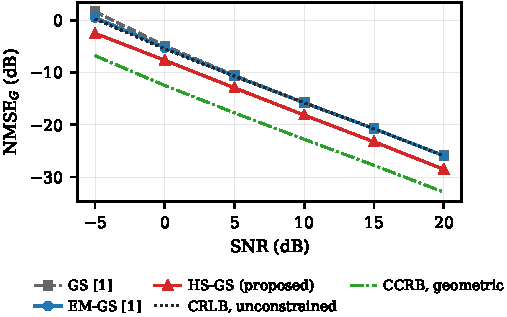
\includegraphics[width=0.62\columnwidth]{fig/fig1_nmse_vs_snr.pdf}
\caption{\textbf{Family B3.} NMSE versus SNR at $N=32$, $K=3$, $P=30$,
RSR $=12$~dB (single-user), $T=50$, $n_{\mathrm{cz}}=4$, $400$ paired trials
per point, ratio-of-sums pooling \eqref{eq:nmse}. EM-GS tracks the rank-one
unconstrained CRLB to within $0.051$~dB above $5$~dB. Neither bound governs a
biased estimator (\S\ref{sec:crlb}-C).}
\label{fig:snr}
\end{figure}

\subsection{Distance to the bounds, and crossings}

HS-GS lies above the geometric CCRB at $34$ of the $36$ family-B3 points, by
% SOURCE: recomputed from results/track_b/b3/*.npz (ratio-of-sums, eq. (13))
% differenced against results/track_b/constrained_crlb.json ["constrained"]["b3"].
% Supersedes the values carried in paper/hsgs.tex (0.32--8.85 / 0.32--1.41 /
% 4.29--4.82), which do not reproduce under either pooling rule.
$0.34$--$9.09$~dB, and the gap \emph{grows} with $N$ ($+0.34$--$1.44$~dB at
$N=8$, $P=30$; $+4.36$--$4.88$~dB at $N=32$, $P=30$): HS-GS captures more structural
gain in absolute terms as the array grows, but a smaller share of what is
available.

Curves do fall below the plotted bounds, in two distinct senses, and neither is
a violation.

\emph{Below the unconstrained CRLB.} HS-GS lies below it at $26$ of $36$
points, by up to $6.94$~dB. That bound governs estimators treating $\bG$ as
$2NK$ free parameters; HS-GS exploits a prior it does not model, so the bound
simply does not apply to it. Its proper reference is the CCRB, respected at
$34$ of $36$.

\emph{Below the CCRB.} The remaining two crossings are consistent with bias, as
\eqref{eq:mse} permits. They occur at the two lowest-SNR points of the smallest
% SOURCE: recomputed from results/track_b/b3/*.npz against
% results/track_b/constrained_crlb.json ["constrained"]["b3"].
aperture --- $N=8$, $P=10$, SNR $-5$ and $0$~dB --- by $2.35$ and $0.15$~dB,
which is where the shrinking update is furthest from unbiased. The baselines
show the same low-SNR pattern and no high-SNR one: GS and EM-GS dip below the
CCRB only at $N=8$, $P=10$, $-5$~dB, by $0.55$ and $0.88$~dB, and stay above it
at every point with SNR $\ge15$~dB (nearest margin $0.84$~dB).

% CAVEAT, load-bearing for the audit: the earlier draft paper/hsgs.tex
% attached shrinkage coefficients c = <Ghat,G>/||G||_F^2 to this paragraph
% (c_EM = 0.944; c_HS = 0.561, 0.776) together with a 2.62 dB crossing figure.
% None of these can be regenerated from the retained stores: the b3 archives
% keep squared-error numerators and the denominator, not inner products, and
% the 2.62 dB figure does not reproduce under either pooling rule. They are
% therefore NOT restated here. Recovering them requires rerunning the sweep.
A per-trial shrinkage diagnostic $c=\langle\hat\bG,\bG\rangle/\|\bG\|_F^{2}$
would make this argument quantitative rather than circumstantial. The retained
\texttt{b3} archives store squared-error numerators only, so $c$ cannot be
recovered from them without rerunning the sweep, and we do not quote it.
\textbf{We do not claim bias accounts for every crossing} --- only that the
observed pattern is consistent with it and that no crossing requires an
estimator to beat a bound that governs it.

% =====================================================================
\section{Aperture Scaling}\label{sec:aperture}
% =====================================================================

This is the result that connects the Fisher analysis to measurement.

\subsection{Principal result (family B3)}

Fig.~\ref{fig:scaling} plots the paired gain against array size. Averaged over
the twelve operating points at each array size --- the six SNR values of
Table~\ref{tab:config} at each of $P\in\{10,30\}$ --- the gain is
% SOURCE: results/track_b/b3/N{8,16,32}_P{10,30}_snr*.npz, 400 trials/point;
% per-operating-point mean, the pooling scripts/plot_paper.py::fig2 draws
\begin{center}
$-0.19$, \quad $+0.78$, \quad $+2.85$~dB \quad at $N=8,16,32$,
\end{center}
with win rates $33.5$, $74.0$, $95.3\%$ and the constraint active in $57.5$,
$92.7$, $99.6\%$ of trials.

\textbf{Under the same averaging EM-GS varies by $0.012$~dB.} This is the
measured counterpart of the block-diagonal Fisher structure of
\S\ref{sec:crlb}-A: the $N$-dependence belongs to the structural prior, not to
a degrading baseline. Had EM-GS itself deteriorated with $N$, the widening gap
would be uninformative.

\begin{figure}[!t]
\centering
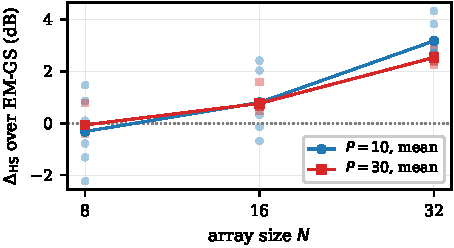
\includegraphics[width=0.62\columnwidth]{fig/fig2_gain_vs_N.pdf}
\caption{\textbf{Family B3.} Paired HS-GS gain over EM-GS versus array size.
$K=3$, RSR $=12$~dB, $T=50$, $n_{\mathrm{cz}}=4$, $400$ trials per point.
Two pilot counts are shown: $P=30$, which Figs.~\ref{fig:snr}
and~\ref{fig:pathcount} also use, and $P=10$ as an auxiliary curve. Faint
markers are the six individual SNR operating points of each curve; solid lines
are their means. The headline $-0.19/+0.78/+2.85$~dB is the mean over all
twelve points (six SNR values $\times$ two pilot counts). At $N=8$ the points
straddle zero, so no single scalar summarises that array size.}
\label{fig:scaling}
\end{figure}

\subsection{$N=8$ is a mixed result, not a small positive one}

At $N=8$ the capacity is $\rmax=4$ while $L_k\in\{3,\dots,7\}$, so the prior is
frequently vacuous or actively harmful: the projection is inactive in $42.5\%$
of trials, and where active it often truncates genuine components.
% SOURCE: results/track_b/b3/N8_P{10,30}_snr*.npz
HS-GS gains $+0.78$ and $+1.47$~dB at $-5$~dB (at $P=30$ and $P=10$
respectively) but turns negative as SNR rises, reaching $-2.23$~dB.

The mechanism is the one \eqref{eq:mse} predicts. Truncation bias does not
shrink with noise. As SNR rises the variance term falls while the bias term
does not, so the trade stops paying and then reverses. \textbf{The sign of any
scalar summary at $N=8$ depends on the pooling}, which is why we report the
per-point values rather than a single number.

\subsection{Extended aperture diagnostic (family EXT --- a separate experiment)}

Family EXT is a \emph{different} experiment: $P=30$ only, seven SNR points
extended down to $-10$~dB, and different trial counts
(Table~\ref{tab:config}). Its numbers must not be substituted for the B3
numbers above, and we report both because they answer different questions ---
B3 gives the paired gain across two pilot counts, EXT gives the absolute NMSE
of each estimator separately.

Fig.~\ref{fig:panels} plots the two absolute NMSE curves. Two facts separate
cleanly.
% SOURCE: trackB_hankel_emgs/results/figure_array_size_comparison.csv
\textbf{EM-GS is flat in $N$}: SNR-averaged $-10.321$, $-10.337$, $-10.301$~dB
at $N=8,16,32$, a spread of $0.036$~dB, and equally flat inside every panel.
\textbf{HS-GS is the only curve that moves}: $-10.350$, $-11.149$,
$-12.753$~dB, so the gap widens monotonically, $0.03\to0.81\to2.45$~dB.

\textbf{These are not the B3 numbers and should not be quoted as such.} The
difference ($0.03/0.81/2.45$ versus $-0.19/+0.78/+2.85$) is fully explained by
configuration: EXT averages seven SNR points including $-10$~dB at one pilot
count, B3 averages twelve points at two pilot counts. Both are internally
consistent; neither is more correct.

In the EXT configuration the $N=8$ sign change is again visible: the
SNR-averaged $0.03$~dB conceals HS-GS gaining $0.744$~dB at $-10$~dB but
losing $0.190$--$0.403$~dB at $0$~dB and above.

\begin{figure}[!t]
\centering
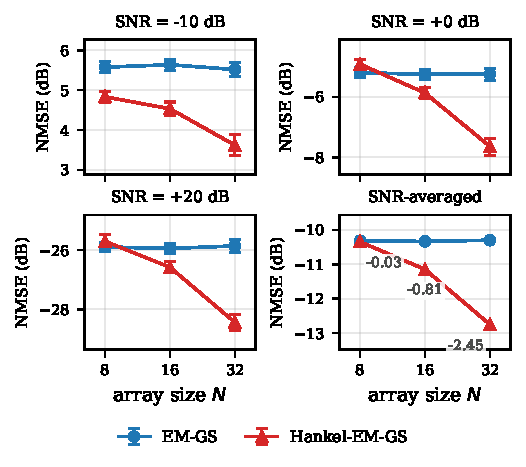
\includegraphics[width=0.68\columnwidth]{fig/fig5_nmse_vs_N_panels.pdf}
\caption{\textbf{Family EXT --- a separate experiment from
Fig.~\ref{fig:scaling}.} Absolute channel NMSE versus array size: three SNR
regimes and, bottom right, the SNR-averaged summary (mean of the seven per-SNR
decibel values, taken \emph{after} conversion; inset labels give HS-GS minus
EM-GS). $K=3$, $P=30$ only, RSR $=12$~dB, $L_k\sim\mathcal{U}\{3..7\}$, SNR
grid extended to $-10$~dB; $600/400/200$ paired trials per point at
$N=8/16/32$; error bars $95\%$ bootstrap.}
\label{fig:panels}
\end{figure}

% =====================================================================
\section{Controlled Path-Count Experiment}\label{sec:pathcount}
% =====================================================================

Every experiment above draws $L_k$ at random, so none isolates path count.
Family EXT fixes $L_k=L$ identically across users and sweeps it to the
capacity.

% SOURCE: trackB_hankel_emgs/results/experiment_C_path_count.csv, gain_db
At $N=32$, $P=30$, SNR $=5$~dB, RSR $=12$~dB, $300$ trials per point, the gain
decays strictly monotonically:
\begin{center}
$7.04$,\ $3.56$,\ $1.79$,\ $1.04$,\ $0.58$,\ $0.27$,\ $0.05$,\ $-0.12$~dB
\quad for $L=2,4,\dots,16$,
\end{center}
with the per-trial win rate falling from $100\%$ to $45.0\%$ and
% SOURCE: same file, em_gs_db column, range 0.191 dB
EM-GS flat to $0.191$~dB across the entire sweep.

\textbf{This is the mechanism test, and it rules out generic denoising.} A
generic denoiser would keep helping at large $L$, where the estimate is exactly
as noisy as at small $L$. Instead the gain vanishes precisely where the prior
becomes vacuous, $L\to\rmax=16$. The flat EM-GS curve confirms the sweep is not
confounded by the baseline changing.

\textbf{Two details, both negative.} The null is reached at $L=14$
($+0.05$~dB, CI $[-0.05,+0.14]$), one grid point \emph{before} the ceiling, and
at $L=16$ the gain is small but significantly \emph{negative}
($-0.12$~dB, CI $[-0.21,-0.04]$). The selector explains this rather than the
theory: mean $\hat L$ reaches only $11.63$ at $L=16$, so the constraint is
still active in $89.3\%$ of trials and there discards genuine components ---
the $\hat L<L$ under-selection regime of \S\ref{sec:method}-D.

\begin{figure}[!t]
\centering
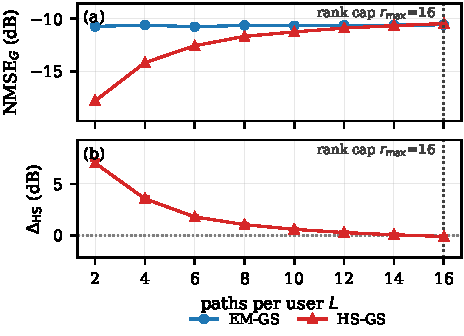
\includegraphics[width=0.62\columnwidth]{fig/fig3_pathcount.pdf}
\caption{\textbf{Family EXT.} Controlled path count: $N=32$, $K=3$, $P=30$,
SNR $=5$~dB, RSR $=12$~dB, $300$ trials per point, $L$ fixed and identical
across users. (a) EM-GS is flat in $L$ --- path count does not affect an
estimator that ignores structure --- while HS-GS rises to meet it. (b) The
paired gain decays monotonically to zero as $L$ approaches
$\rmax=\lceil N/2\rceil=16$; the $95\%$ paired bootstrap band is plotted but is
narrower than the markers. The hypothesis was recorded before the experiment
was run.}
\label{fig:pathcount}
\end{figure}

% =====================================================================
\section{Structural Spectrum Diagnostic}\label{sec:spectrum}
% =====================================================================

Fig.~\ref{fig:spectrum} shows, for one illustrative realisation, why the prior
exists and what the projection actually achieves.

The true channel's Hankel spectrum falls to $\sim\!10^{-16}$ immediately after
index $L$: the low-rank property is exact, as \eqref{eq:rank} states. The EM-GS
estimate has no such cliff --- noise fills the spectrum, so the estimate is not
a sum of $L$ exponentials and does not lie in $\mathcal{S}_L$. After four
Cadzow sweeps a cliff reappears at the correct index, but only to
$\sim\!10^{-3}$.

That shortfall is the concrete measure of \eqref{eq:notproj} being an
approximate rather than exact projection, and it upper-bounds how much
structure the method can impose --- consistent with HS-GS attaining only part
of the CCRB headroom (\S\ref{sec:bounds}-B).

\textbf{Caveat.} This is one realisation chosen for illustration. It shows the
qualitative mechanism; it is not a statistical claim about the magnitude of the
residual, and we do not use it as one.

\begin{figure}[!t]
\centering
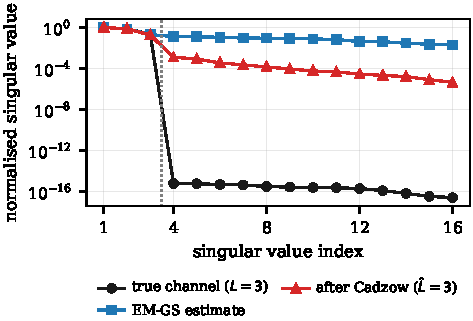
\includegraphics[width=0.62\columnwidth]{fig/fig4_hankel_spectrum.pdf}
% SOURCE: trackB_hankel_emgs/results/diagnostic_spectrum.json (family EXT tree,
% trial 0, master_seed 20250820, L_hat forced to true L, cadzow_iter 4).
% true_channel[3] = 5.73e-16; em_gs_estimate[3] = 0.1304; after_cadzow[3] = 1.24e-3.
\caption{\textbf{Family EXT, single illustrative realisation.}
Normalised Hankel singular values for one channel column, $N=32$, $L=3$,
SNR $=5$~dB, RSR $=12$~dB, $n_{\mathrm{cz}}=4$, order forced to the true $L$.
The true channel is exactly rank $L$ ($\sigma_4/\sigma_1=5.7\times10^{-16}$),
the EM-GS estimate is full numerical rank ($\sigma_4/\sigma_1=0.130$), and four
Cadzow sweeps restore the cliff only approximately, to $1.2\times10^{-3}$.}
\label{fig:spectrum}
\end{figure}

% =====================================================================
\section{From Path Count to Effective Rank}\label{sec:effrank}
% =====================================================================

\S\ref{sec:pathcount} establishes the mechanism in terms of the generator
parameter $L$. That parameter has two defects as a general coordinate.

First, \textbf{$L$ is not a property of a channel} but of the process that
produced it; a receiver cannot measure it, and two generators with the same $L$
need not produce equally compressible liftings. Second, and decisively,
\textbf{$L$ mispredicts}: a $16$-path channel on a $32$-element array is
algebraically full rank, so raw path count says the prior is vacuous, yet its
% SOURCE: reports/trackD_normalization.md A2, via scratch/trackD_partA9_normalization.py
effective Hankel rank is $8.73$ and the lifting is in fact compressible.
Closely spaced paths (\S\ref{sec:hankel}) produce exactly this situation.

We therefore replace $L$ by a spectral measure. For singular values $\sigma_i$
of $\Hank(\bg)$ define $p_i=\sigma_i/\sum_j\sigma_j$ and the Roy--Vetterli
effective rank \cite{royvetterli2007}
\begin{equation}\label{eq:reff}
\reff=\exp\Bigl(-\sum_i p_i\log p_i\Bigr),
\end{equation}
normalised by the capacity \eqref{eq:cap} to give the dimensionless coordinate
\begin{equation}\label{eq:rho}
\rho=\reff/\rmax .
\end{equation}

\textbf{$\reff$ must be computed on the noiseless channel.} The effective rank
of the \emph{estimate} is set by the noise floor, not by the channel: it was
measured at $8.91$--$11.77$ across $L=1\dots16$ at $5$~dB,
% SOURCE: reports/trackD_spectral_diagnostics.json (PROMPT 8 diagnostic C1)
which would collapse every configuration onto essentially one point and destroy
the coordinate. This is a diagnostic quantity computed from a known channel,
not something a receiver estimates online.

Fig.~\ref{fig:rawL} shows the path-count sweep on the raw $L/\rmax$ axis for
comparison with the re-indexed version in Fig.~\ref{fig:boundary}. Re-indexing
the same sweep by $\rho$ moves the zero crossing from $L/\rmax=0.90$ to
% SOURCE: reports/trackD_normalization.md A2 re-indexing
$\rho=0.518$, and turns a statement about one simulator's $L$ values into one
about any channel: the useful region is $\rho\lesssim0.5$.

\begin{figure}[!t]
\centering
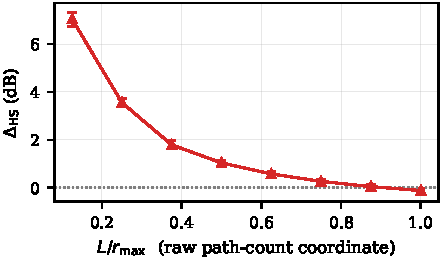
\includegraphics[width=0.62\columnwidth]{fig/fig6_gain_vs_raw_L.pdf}
\caption{\textbf{Family EXT.} The controlled path-count sweep of
Fig.~\ref{fig:pathcount} plotted against the \emph{raw} coordinate $L/\rmax$
($N=32$, $\rmax=16$, $P=30$, SNR $=5$~dB, RSR $=12$~dB, $300$ trials per
point; error bars $95\%$ paired bootstrap). Compare Fig.~\ref{fig:boundary},
where the same physical effect is indexed by effective rank and becomes
comparable across array sizes.}
\label{fig:rawL}
\end{figure}

% =====================================================================
\section{Array-Invariant Effective-Rank Boundary}\label{sec:boundary}
% =====================================================================

If $\rho$ is the right coordinate, curves measured at different array sizes
should line up on it. Family TD tests this at $N\in\{16,32,64\}$
(Fig.~\ref{fig:boundary}).

\textbf{The sign boundary is stable.} The zero crossings are
% SOURCE: reports/trackD_partB9_analysis.json, B1_collapse.zero_crossing_r_eff_over_cap
$\rho=0.588$, $0.518$, $0.544$ at $N=16,32,64$ --- a spread of $0.070$ across a
fourfold change in aperture. Within the tested range, $\rho\approx0.5$ locates
where the prior stops paying, irrespective of array size.

\textbf{The gain magnitude does not collapse, and we state the residual rather
than report a collapse.} Over the $\rho$ window both arrays cover, $N=16$ lies
above $N=64$ by
% SOURCE: same file, B1_collapse.PRIMARY_internal_N16_vs_N64
a mean of $0.493$~dB and a maximum of $0.901$~dB, one-signed throughout and
monotone in $N$. \textbf{We have no account of this residual.} One candidate is
pencil quantisation at small capacity --- $\rmax(16)=8$ admits eight distinct
ranks against $32$ at $N=64$, so the selector's grid is coarser --- but that is
untested, and the experiment that would settle it is a pencil sweep at fixed
$N$.

\textbf{Two of the three crossings are extrapolated.} Neither $N=16$ nor
$N=64$ has a measured cell whose gain is actually negative; their crossings are
obtained by extending the last two measured points. Only the $N=32$ crossing is
bracketed by a measured sign change.
% SOURCE: same file, B1_collapse.zero_crossing_is_bracketed_not_extrapolated

\textbf{What we therefore claim.} This is an \emph{empirical effective-rank
relation} over the tested array sizes and channel families. It is not a scaling
law, it is not universal, and the imperfect magnitude collapse is a genuine
limitation rather than a rounding detail.

\begin{figure}[!t]
\centering
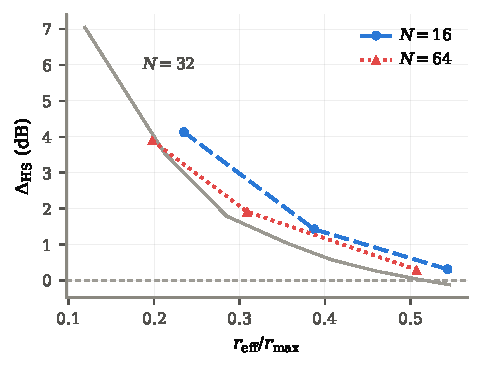
\includegraphics[width=0.62\columnwidth]{fig/fig7_boundary_invariance.pdf}
\caption{\textbf{Family TD.} $\dhs$ against $\rho=\reff/\rmax$ for
$N\in\{16,32,64\}$. $K=3$, $P=20$, RSR $=10$~dB, $T=100$, $n_{\mathrm{cz}}=1$,
adaptive order, SNR $\sim\mathcal{U}[-10,20]$~dB, paired per-trial median;
$83$--$874$ trials per cell. The grey curve is the re-indexed $N=32$ relation.
The sign boundary is stable to within $0.070$ in $\rho$; the gain
\emph{magnitude} is not, with a one-signed residual of mean $0.493$~dB
(max.\ $0.901$~dB) between $N=16$ and $N=64$.}
\label{fig:boundary}
\end{figure}

% =====================================================================
\section{Prospective Cross-Generator Validation}\label{sec:crossgen}
% =====================================================================

\subsection{Chronology, and what makes this prospective}

An earlier stage of this work concluded that robustness under clustered
propagation was not established and named the decisive next experiment:
\emph{repeat the principal comparison under a clustered generator --- a
falsification test, not a confirmation exercise.} This section is that test,
run twice.

The order of operations matters and was enforced by version control. For each
new generator: (i) $\reff$ was measured on its noiseless channels and $\rho$
computed; (ii) a predicted $\dhs$ was read off the relation and
\textbf{committed to the repository}; (iii) only then was the estimator run.
\textbf{The relation was not refitted after any measurement.}

\subsection{The prediction rule, stated so it can be reproduced}

The relation is the eight-point table of $(\rho,\dhs)$ pairs obtained by
re-indexing the path-count sweep of \S\ref{sec:pathcount}. The predicted
$\dhs$ is its \textbf{piecewise-linear interpolation} at the measured $\rho$
--- \texttt{numpy.interp} on those eight points.
% SOURCE: scratch/trackD_step0_cui_predict.py:73 (np.interp) and :78 (interval)
\textbf{No curve is fitted}: there is no regression, no spline, no parametric
form. The prediction interval is that same interpolation evaluated at the
interquartile endpoints of $\reff$ over the channel realisations, so it
reflects channel variability rather than being asserted.

\subsection{Terminology: cross-generator, not out-of-model}

Both validation generators produce receive-side ULA channels that are sums of
spatial complex exponentials, i.e.\ they still satisfy \eqref{eq:chan}. What
differs is the \emph{distribution} over $(L_k,\alpha_{\ell,k},\theta_{\ell,k})$
--- clustered rather than uniform angles, a different path count, different
gain statistics. We therefore call these \textbf{cross-generator} or
distribution-shift tests. Calling them ``out-of-model'' would overstate what is
being tested: the mathematical family is unchanged.

This does not weaken the result. The relation was fitted using one
channel-generation distribution and tested prospectively, without refitting, on
previously unseen channel-generation distributions.

\subsection{Results}

Table~\ref{tab:predictions} and Fig.~\ref{fig:crossgen} give the outcome.

% SOURCE: reports/trackD_partB9_analysis.json, B6_xiao.B6_xiao_clustered
\textbf{Clustered Saleh--Valenzuela} \cite{meijerink2014}. At $\rho=0.331$ the
relation predicts $+1.30$~dB. Measured: $+1.173$~dB, CI $[+1.017,+1.380]$ ---
an error of $0.13$~dB, with the prediction inside the measured interval.

% SOURCE: reports/trackD_step0_cui_prediction.json and partB9_analysis.json B8_cui_measured
\textbf{A second, independently specified configuration} \cite{precoding2408}:
the receive-side Saleh--Valenzuela configuration of a precoding study by the
same group as \cite{cui2025} --- $L=10$ paths, $\alpha_\ell\sim\CN(0,1)$,
angles $\mathcal{U}(-90^\circ,90^\circ)$. Only the channel configuration is
borrowed; that work is not a competing estimator, and it uses ULAs at both ends
with incident and departure angles, of which we use the receive side only. At
$\rho=0.400$ the relation predicts $+0.648$~dB with interval
$[+0.367,+1.015]$. Measured: $+0.963$~dB, CI $[+0.808,+1.086]$.

\textbf{The prediction error here is $0.315$~dB} --- inside the registered
interval and on the correct side of zero, but substantially larger than the
first. We report it as such and not as a second $0.13$~dB hit. Together the two
bound what the relation is good for: it places an unseen generator on the
correct part of the curve, and it is \emph{not} accurate to a tenth of a
decibel in general.

% SOURCE: reports/trackD_partB9_analysis.json, B6_xiao.B6_xiao_literal
\textbf{A third reading, and a partial match.} Interpreting the clustered
specification literally --- all $40$ rays drawn independently rather than in
clusters --- raises $\rho$ to $0.748$, where the relation predicts a small
negative gain, $-0.12$~dB. The measured median is exactly $0.000$~dB. The
magnitude is right to $0.12$~dB, but \emph{the mechanism is not the predicted
one}: rather than degrading, the order selector declines to project at all in
$29.1\%$ of trials, against $1.4\%$ on the clustered model and $1.5\%$ on the
second configuration. The rule discriminates between generators without being
told which it faces. We record this as a partial match.

\textbf{Clustering did not eliminate the gain}, which the earlier stage had
identified as a live possibility.

\begin{table}[!t]
\caption{Prospective predictions against measurements. Each prediction was
committed to version control before the corresponding measurement was run, and
the relation was not refitted afterwards. Family TD configuration.}
\label{tab:predictions}
\centering
\footnotesize
\setlength{\tabcolsep}{3.5pt}
\begin{tabular}{lccccc}
\toprule
Generator & $\rho$ & Pred. & Meas. & CI$_{95}$ & Err. \\
\midrule
% SOURCE: reports/trackD_partB9_analysis.json
Clustered SV \cite{meijerink2014} & $0.331$ & $+1.30$ & $+1.173$ &
$[1.017,1.380]$ & $0.13$ \\
$L=10$ cfg.\ \cite{precoding2408} & $0.400$ & $+0.648$ & $+0.963$ &
$[0.808,1.086]$ & $\mathbf{0.315}$ \\
Literal reading & $0.748$ & $-0.12$ & $0.000$ & degen. & $0.12$ \\
\bottomrule
\end{tabular}
\end{table}

\begin{figure}[!t]
\centering
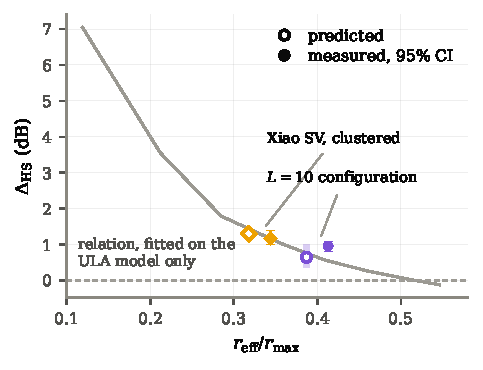
\includegraphics[width=0.62\columnwidth]{fig/fig8_cross_generator.pdf}
\caption{\textbf{Family TD.} Predictions registered before measurement, against
measurement. $N=32$, $K=3$, $P=20$, RSR $=10$~dB, adaptive order,
$n_{\mathrm{cz}}=1$, SNR $\sim\mathcal{U}[-10,20]$~dB; $266$--$276$ trials per
generator. Both generators produce channels of the form \eqref{eq:chan}; what
differs is the distribution over $(L_k,\alpha_{\ell,k},\theta_{\ell,k})$. The
relation was fitted on the generator of \S\ref{sec:pathcount} alone and not
refitted afterwards.}
\label{fig:crossgen}
\end{figure}

% =====================================================================
\section{User Count and $K$-Invariance}\label{sec:kinv}
% =====================================================================

Equation \eqref{eq:compress} showed $K$ cancelling from the compression ratio,
motivating the hypothesis that $\dhs$ is invariant in $K$. Testing it requires
care: sweeping $K$ at fixed $P$ would simultaneously change \emph{pilot
adequacy} $P/2K$ and confound the two effects. We therefore hold $P/2K=3.33$
fixed, using $P=13,20,27$ at $K=2,3,4$.

% SOURCE: reports/trackD_partB9_analysis.json, B2_K_invariance and cells B2_*
The outcome is genuinely mixed and we report it that way
(Fig.~\ref{fig:kinv}).

\textbf{At SNR $\ge5$~dB the invariance holds well}: $\dhs$ spans
$+3.563$ to $+3.658$~dB across $K\in\{2,3,4\}$, a spread of $0.095$~dB.

\textbf{Pooled over all SNR it does not}: the spread is $0.294$~dB and is
monotone in $K$ ($+3.403$, $+3.161$, $+3.109$~dB). Our pre-registered falsifier
was a monotone trend exceeding $0.3$~dB, \textbf{which this misses by
$0.006$~dB}. We do not present that as a pass. The adjacent-pair confidence
intervals overlap throughout, so no individual step is significant, and the
pooled trend is driven by the bins below $0$~dB where each cell contributes
roughly $45$ trials.

\textbf{The honest statement} is that the DoF cancellation transfers to
estimation performance at moderate and high SNR, that below $0$~dB there is a
decline with $K$ of about $0.3$~dB that \eqref{eq:compress} does not predict,
and that the low-SNR evidence is thin enough to warrant re-measurement before
being believed.

\begin{figure}[!t]
\centering
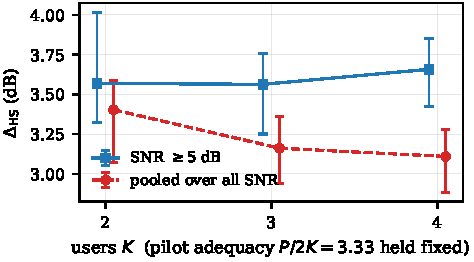
\includegraphics[width=0.62\columnwidth]{fig/fig9_k_invariance.pdf}
\caption{\textbf{Family TD.} $\dhs$ against user count at \emph{fixed} pilot
adequacy $P/2K=3.33$ ($P=13,20,27$ at $K=2,3,4$). $N=32$, RSR $=10$~dB,
$T=100$, $n_{\mathrm{cz}}=1$, adaptive order, SNR $\sim\mathcal{U}[-10,20]$~dB;
$245$--$306$ trials per cell; paired per-trial median with $95\%$ bootstrap
intervals. The high-SNR spread is $0.095$~dB; pooled over all SNR it is
$0.294$~dB and monotone, missing the pre-registered $0.3$~dB falsifier by
$0.006$~dB.}
\label{fig:kinv}
\end{figure}

% =====================================================================
\section{Summary of Quantitative Findings}\label{sec:summary}
% =====================================================================

Table~\ref{tab:summary} collects the principal numbers with their experiment
family, so that no result is read against the wrong configuration.

\begin{table*}[!t]
\caption{Principal quantitative findings, each tagged with its experiment
family (Table~\ref{tab:config}). Numbers from different families are not
comparable as measurements of the same estimator.}
\label{tab:summary}
\centering
\begin{tabular}{lllc}
\toprule
Finding & Value & Family & Section \\
\midrule
Hankel capacity & $\rmax(N)=\lceil N/2\rceil$ & derivation & \ref{sec:hankel} \\
Rank-two error in the bound & $0.17$--$4.64$~dB too low & B3 (36 pts) & \ref{sec:crlb} \\
EM-GS vs unconstrained CRLB, SNR $\ge5$ & within $0.051$~dB & B3 & \ref{sec:bounds} \\
EM-GS vs CRLB at $-5$ / $0$~dB & $0.295$ / $0.237$~dB & B3 & \ref{sec:bounds} \\
CCRB below unconstrained CRLB & $7.05$--$7.11$~dB & B3 & \ref{sec:bounds} \\
HS-GS over EM-GS, $N=32$, $P=30$ & $+2.27$ to $+3.04$~dB & B3 & \ref{sec:bounds} \\
Aperture gain, $N=8/16/32$ & $-0.19$ / $+0.78$ / $+2.85$~dB & B3 (12 pts) & \ref{sec:aperture} \\
EM-GS flatness in $N$ & $0.012$~dB & B3 (12 pts) & \ref{sec:aperture} \\
Win rate, $N=8/16/32$ & $33.5$ / $74.0$ / $95.3\%$ & B3 & \ref{sec:aperture} \\
Constraint active, $N=8/16/32$ & $57.5$ / $92.7$ / $99.6\%$ & B3 & \ref{sec:aperture} \\
Aperture gap (separate experiment) & $0.03$ / $0.81$ / $2.45$~dB & \textbf{EXT} & \ref{sec:aperture} \\
EM-GS flatness (separate experiment) & $0.036$~dB & \textbf{EXT} & \ref{sec:aperture} \\
Path-count decay, $L=2\to16$ & $7.04\to-0.12$~dB & EXT & \ref{sec:pathcount} \\
EM-GS flatness in $L$ & $0.191$~dB & EXT & \ref{sec:pathcount} \\
Effective-rank zero crossings & $0.588$ / $0.518$ / $0.544$ & TD & \ref{sec:boundary} \\
Magnitude residual, $N=16$ vs $64$ & mean $0.493$, max $0.901$~dB & TD & \ref{sec:boundary} \\
Prospective error, generator 1 / 2 & $0.13$ / $\mathbf{0.315}$~dB & TD & \ref{sec:crossgen} \\
Abstention, clustered / literal & $1.4\%$ / $29.1\%$ & TD & \ref{sec:crossgen} \\
$K$-invariance, SNR $\ge5$ / pooled & $0.095$ / $0.294$~dB & TD & \ref{sec:kinv} \\
Runtime vs chained EM-GS & $1.49$ / $1.32$ / $1.22\times$ & B3 & \ref{sec:complexity} \\
Order-selection share of runtime & $57.7$--$85.5\%$ & B3 & \ref{sec:complexity} \\
\bottomrule
\end{tabular}
\end{table*}

% =====================================================================
\section{Discussion}\label{sec:discussion}
% =====================================================================

The experiments are not a list; they build on one another, and it is worth
saying explicitly which statements are derived, which are observed, and which
are interpretation.

\textbf{Derived.} The rank bound \eqref{eq:rank}, the capacity \eqref{eq:cap},
the compression ratio \eqref{eq:compress}, the rank-one form of the Fisher
information \eqref{eq:fisher}, and its block diagonality across receive
elements. These follow from the model and require no measurement.

\textbf{Observed.} That HS-GS improves on EM-GS where the lifting is
compressible; that the improvement grows with aperture while EM-GS does not
move; that the gain decays to zero exactly as $L\to\rmax$; that the sign
boundary sits near $\rho\approx0.5$ across three array sizes; that two
prospective predictions landed within $0.13$ and $0.315$~dB; that $K$-invariance
holds at high SNR and not pooled.

\textbf{Interpretation.} The following is our reading, not a proof. The
path-count experiment establishes that HS-GS benefits from Hankel
compressibility rather than from generic denoising --- the vanishing of the
gain at the capacity is the discriminating observation. Effective rank then
generalises that from a generator parameter to realised spectral complexity,
which is what allows the relation to be carried to a generator it was not
fitted on. The aperture result is explained by the two moving in opposite
directions: $\rmax=\lceil N/2\rceil$ grows with the array while the channel's
effective complexity need not, so $\rho$ falls and the prior becomes more
informative. Finally, the Fisher analysis is what licenses attributing this to
cross-element structure rather than to EM-GS degrading with $N$ --- and the
measured $0.012$~dB flatness is the empirical check on that attribution.

\textbf{What would falsify the picture.} If a cross-element prior with no
Hankel structure produced the same aperture scaling, the mechanism claim would
need revision. If the magnitude residual of \S\ref{sec:boundary} turned out to
scale with something other than pencil quantisation, $\rho$ would be incomplete
as a coordinate. If a generator with $\rho\ll0.5$ produced no gain, the
relation would be refuted outright; none of the three tested did.

% =====================================================================
\section{Limitations}\label{sec:limits}
% =====================================================================

Stated as a list of what has and has not been demonstrated.

\begin{enumerate}
\item \textbf{Simulation only.} No measured hardware, no recorded channel data.
\item \textbf{No hardware channel.} The atomic response is modelled through
\eqref{eq:obs}; non-idealities of a physical vapour cell are absent.
\item \textbf{Geometric ULA dependence.} All results assume \eqref{eq:chan};
the cross-generator tests change the distribution but not the family.
\item \textbf{$N=8$ fails at high SNR.} The gain is negative above $0$~dB and
the array-size result there is mixed, not weakly positive.
\item \textbf{Hard rank truncation is biased.} The bias does not vanish as
noise decreases, which is exactly why $N=8$ degrades at high SNR.
\item \textbf{One shared scalar rank for $K$ users.} The selector applies a
single $\hat L$ to all columns despite their differing true orders.
\item \textbf{Finite Cadzow sweeps.} Four sweeps leave a measurable residual
(\S\ref{sec:spectrum}); the structure is imposed only approximately.
\item \textbf{Non-convex structured projection.} The intersection of the rank
and Hankel sets is a non-convex variety and \eqref{eq:notproj} is not an exact
idempotent projection onto it.
\item \textbf{No convergence guarantee} for the outer iteration
\eqref{eq:map}, and we claim none.
\item \textbf{The effective-rank magnitude does not collapse across $N$}: a
one-signed residual of mean $0.493$~dB, maximum $0.901$~dB, unexplained.
\item \textbf{Two of three zero crossings are extrapolated}, not bracketed by a
measured sign change.
\item \textbf{The $K$-invariance pooled criterion narrowly fails}, missing the
pre-registered falsifier by $0.006$~dB.
\item \textbf{The second prospective prediction errs by $0.315$~dB}, an order
of magnitude worse than the first.
\item \textbf{The bounds do not govern the estimators compared to them.} CRLB
and CCRB constrain unbiased estimators; every estimator here is biased.
\item \textbf{Cross-generator tests remain inside the ULA
sum-of-exponentials family.} They are distribution shifts, not model
violations.
\item \textbf{Equal user power throughout.} Near--far effects are untested.
\item \textbf{Limited array sizes and channel families}: $N\in\{8,16,32\}$
(B3, EXT) and $\{16,32,64\}$ (TD); three generators.
\item \textbf{Order selection dominates runtime} ($57.7$--$85.5\%$), and no
attempt has been made to reduce it.
\item \textbf{The bias explanation of the CCRB crossings is circumstantial.}
The retained \texttt{b3} archives store squared-error numerators only, so the
per-trial shrinkage $c=\langle\hat\bG,\bG\rangle/\|\bG\|_F^{2}$ that would make
the argument quantitative cannot be recovered without rerunning the sweep
(\S\ref{sec:bounds}-B). An earlier draft quoted such coefficients; they are not
reproducible from the stores retained here and are not restated.
\end{enumerate}

% =====================================================================
\section{Conclusion}\label{sec:conclusion}
% =====================================================================

The progression of this work is short to state.

Magnitude-only reception makes multi-user channel estimation a biased
phase-retrieval problem. Under the unconstrained row-wise parameterisation of
that problem the Fisher information is block diagonal across receive elements,
so normalised per-element information does not grow with the array and an
unstructured estimator gains nothing from aperture --- which we then measure,
at $0.012$~dB of movement across a fourfold change in $N$. Exploiting aperture
therefore requires cross-element structure, and the geometric ULA model
supplies one: each path contributes a single spatial exponential, so the Hankel
lifting of each column has rank at most the path count. Enforcing that rank
inside the exact iteration, with the order chosen from held-out pilots, yields
$-0.19$, $+0.78$, $+2.85$~dB at $N=8,16,32$ and $2.27$--$3.04$~dB at $N=32$,
$P=30$ against a benchmark the baseline tracks to $0.051$~dB.

A controlled path-count sweep establishes that this is structural rather than
generic denoising, since the gain vanishes precisely where the prior becomes
vacuous. Replacing raw path count by effective Hankel rank relative to capacity
generalises the mechanism from a generator parameter to a measurable property
of a channel, giving an empirical sign boundary near $\rho\approx0.5$ that is
stable to within $0.070$ across $N\in\{16,32,64\}$ --- though the gain
magnitude does not collapse onto that axis, and we report the residual rather
than the collapse. Used prospectively, with predictions committed before
measurement and no refitting, that relation placed two previously unused
channel generators on the correct part of the curve, to within $0.13$ and
$0.315$~dB.

The claims are scoped accordingly. This is an empirical relation over the
tested array sizes and channel families, not a law; the tested generators are
distribution shifts within the ULA sum-of-exponentials family, not departures
from it; the outer iteration has no convergence guarantee; the baseline is not
efficient, only numerically close to a bound that does not strictly govern it;
and the constrained bound is not a lower bound on the mean-squared error of a
biased structured estimator. What has been demonstrated is that a measurable
structural coordinate predicts, before the fact, when this prior is worth
applying.

\bibliographystyle{IEEEtran}
\bibliography{refs}

\end{document}
